\documentclass[11.5pt, twoside, a4paper, titlepage]{report}
\usepackage{graphicx, amssymb, amsmath, mathtools, amsthm}
\usepackage{tikz}
\usetikzlibrary{automata, arrows}
\providecommand{\abs}[1]{\lvert#1\rvert}
\providecommand{\equ}[0]{\begin{equation*}}
\providecommand{\eequ}[0] {\end{equation*}}
\providecommand{\bb}[1]{\mathbb{#1}}
\theoremstyle{definition}
\newtheorem{mydef}{Definition}[section]
\newtheorem{rem}[mydef]{Remark}
\newtheorem{note}[mydef]{Notation}
\newtheorem{eg}[mydef]{Example}
\theoremstyle{plain}
\newtheorem{lem}[mydef]{Lemma}
\newtheorem{thm}[mydef]{Theorem}
\newtheorem{cor}[mydef]{Corollary}
\newtheorem{prop}[mydef]{Proposition}



\begin{document}
\title{Representation of Quivers}
\author{Chanelle Lee \\Student ID: 200646370\\Supervisor: William Crawley-Boevey}
\date{\today}
\maketitle


\tableofcontents

\chapter{Introduction}

\chapter{Homological Algebra}
\section{Chain Complexes}

\begin{mydef}
A \emph{chain complex} $\mathbf{C}_{\bullet}$ consists of a sequence of $\mathbb{R}$-modules $C_i$ ($i \in \mathbb{Z}$) and morphisms of the form,
\begin{equation*}
\mathbf{C}: \qquad \dots \xrightarrow{\delta_{3}} C_2 \xrightarrow{\delta_{2}} C_1 \xrightarrow{\delta_{1 }} C_0 \xrightarrow{\delta_0} C_{-1} \xrightarrow{\delta_{-1}} C_{-2} \xrightarrow{\delta_{-2}}\dots
\end{equation*}
such that $\delta_{n-1}\delta_{n}=0$ for all $n$, i.e. the composition of any two consecutive maps is zero. The maps $\delta_n$ are called the \emph{differentials} of $C$.
\end{mydef}

\begin{rem}
It is convention that the map $\delta_n$ starts at $C_n$.
\end{rem}

\begin{eg}
If we have a field $K$ then we can create the following chain complex:
\begin{equation*}
\mathbf{C}: \qquad \dots \xrightarrow{} 0 \xrightarrow{} K^2 \xrightarrow{\Bigl(\begin{smallmatrix}1&2\\ 3&0\\ 0&0 \end{smallmatrix}\Bigr)} K^3 \xrightarrow{(\begin{smallmatrix}0 & 0 &1\end{smallmatrix})} K \xrightarrow{} 0 \xrightarrow{}\dots
\end{equation*}
We can clearly see that the maps uphold the $\delta^2=0$ condition as,
\begin{equation*}
\begin{pmatrix}0 & 0 &1
\end{pmatrix}
\begin{pmatrix}
1 & 2 \\
3 & 0\\
0 & 0
\end{pmatrix}
=\begin{pmatrix}
0 & 0
\end{pmatrix}.
\end{equation*}
\end{eg}

\begin{eg} \label{Kchaineg}
If we consider the sequence, 
\equ 
\dots \xrightarrow{} 0 \xrightarrow{} K \xrightarrow{\big(\begin{smallmatrix} 1\\ 0 \end{smallmatrix}\big)} K^2 \xrightarrow{(\begin{smallmatrix}1 & 0 \end{smallmatrix})} K \xrightarrow{} 0 \xrightarrow{} \dots
\eequ
however,
\equ
\begin{pmatrix}
1 & 0
\end{pmatrix}
\begin{pmatrix*}
1\\
0
\end{pmatrix*}
= 1 \neq 0.
\eequ
Hence, $\delta^2 \neq0$ and so the sequence is not a chain complex. However, if we change the second map slightly we obtain the chain complex,
\equ
\mathbf{C}: \qquad \dots \xrightarrow{} 0 \xrightarrow{} K \xrightarrow{\big(\begin{smallmatrix} 1\\ 0 \end{smallmatrix}\big)} K^2 \xrightarrow{(\begin{smallmatrix}0 & 1 \end{smallmatrix})} K \xrightarrow{} 0 \xrightarrow{} \dots
\eequ
since, 
\equ
\begin{pmatrix}
1 & 0
\end{pmatrix}
\begin{pmatrix*}
0\\
1
\end{pmatrix*}
= 1 \neq 0.
\eequ
\end{eg}

\begin{mydef}
If $\mathbf{C}$ is a chain complex then its \emph{homology} is defined to be,
\begin{equation*}
H_n(\mathbf{C})=\frac{Ker(\delta_n:C_n \rightarrow C_{n-1})}{Im(\delta_{n+1}:C_{n+1} \rightarrow C_n)} =\frac{Z_n(\mathbf{C})}{B_n(\mathbf{C})}.
\end{equation*}
This becomes an $\mathbb{R}$-module and, since $\delta^2$, it follows that $B_n(\mathbf{C})\subseteq Z_n(\mathbf{C})$.
\end{mydef}

The following Lemma is the solution to Exercise 6.1 in \cite{Rotman}.

\begin{lem}
If $\mathbf{C}$ is a chain complex with $C_n=0$ for some $n$ then $H_n(\mathbf{C})=0$.
\end{lem}
\begin{proof}
Well suppose we have such a chain complex, 
\equ
\mathbf{C}: \qquad \dots \xrightarrow{} C_{n+1} \xrightarrow{\delta_{n+1}} 0 \xrightarrow{\delta_n} C_{n-1} \xrightarrow{} \dots
\eequ
the the homology is,
\equ
H_n(\mathbf{C})=\frac{Ker(\delta_n: 0 \to C_{n-1}}{Im(\delta_{n+1}: C_{n+1}\to 0)},
\eequ
as the only element in $C_n$ is the zero element, and so, $H_n(\mathbf{C})=0$, as required.\\
\end{proof}

Examples \ref{chainMeg} and \ref{chainZeg} are taken from \cite{CB1} and are included here because they are felt to be the clearest at demonstrating a chain complex and homology, however, the more general statement of the second example is presented as Proposition \ref{chainhomprop} because it is an interesting result.

\begin{eg}
 \label{chainMeg}
 If we take a module $M$ then we can make a chain complex;
\begin{equation*}
\mathbf{C}: \qquad \dots \xrightarrow{} 0 \xrightarrow{} M \xrightarrow{} 0 \xrightarrow{} \dots
\end{equation*}
where $M$ is at degree $n$. Then the homology will be:
\begin{equation*}
H_i(\mathbf{C})=\begin{cases}
\frac{Ker(M \rightarrow 0)}{Im(0 \rightarrow M)}=M & i=n,\\
0 & \text{otherwise}.
\end{cases}
\end{equation*}
\end{eg}

\begin{prop}  \label{chainhomprop}
If we have a module homomorphism between $R$-modules, $f: M \xrightarrow{} N$, the we get the chain complex,
\equ
\mathbf{C}: \qquad \underset{\text{deg}}{\dots} \xrightarrow{}\underset{n+2}{0} \xrightarrow{} \underset{n+1}{M} \xrightarrow{f}\underset{n}{N} \xrightarrow{} \underset{n-1}{0} \xrightarrow{}\dots ,
\eequ
and the homology becomes,
\equ
H_i(\mathbf{C})=
\begin{cases}
\frac{N}{Im(f)}=Coker(f) & i=n\\
Ker(f) & i=n+1\\
0 & \text{otherwise}.
\end{cases}
\eequ
\end{prop}
\begin{proof}
Firstly, at degree $n$ we have that,
\equ
H_n(\mathbf{C})=\frac{Ker(N\xrightarrow{}0)}{Im(M\xrightarrow{f}N)}=\frac{N}{Im(f)}=Coker(f).
\eequ
Then at degree $n+1$ we have that,
\equ
H_{n+1}(\mathbf{C})=\frac{Ker(M\xrightarrow{f}N)}{Im(0\xrightarrow{}M)}=Ker(f).
\eequ
Finally, it is clear that everywhere else there is no homology.
\end{proof}

\begin{note}
Here, 
\equ
Coker(f)= \frac{\text{Codomain of }f}{\text{Image of }f},
\eequ
is the \emph{cokernel} of the map $f$.
\end{note}

\begin{eg} \label{chainZeg}
We can have a chain complex of $\mathbb{Z}$-modules,
\equ
\mathbf{C}: \qquad \underset{\text{deg}}{\dots} \xrightarrow{}\underset{2}{0} \xrightarrow{} \underset{1}{\mathbb{Z}} \xrightarrow{a}\underset{0}{\mathbb{Z}} \xrightarrow{} \underset{-1}{0} \xrightarrow{}\dots 
\eequ
where the map $a$ is right multiplication by some $a \in \mathbb{Z}$. The homology is,
\equ
H_i(\mathbf{C}) = 
\begin{cases}
\frac{Ker(\mathbb{Z}\xrightarrow{} 0)}{Im(\mathbb{Z}\xrightarrow{a}\mathbb{Z})}=\frac{\mathbb{Z}}{a\mathbb{Z}} & i=0,\\
0 & \text{otherwise}.
\end{cases}
\eequ
Note that,
\equ
H_0(C)=\frac{\bb{Z}}{a\bb{Z}}= \frac{\text{Codomain of }f}{\text{Image of }f}=Coker(a).
\eequ
Also,
\equ
H_1(C)=\frac{Ker(\bb{Z}\xrightarrow{a}\bb{Z})}{Im(0\xrightarrow{}\bb{Z})}=Ker(a)=0,
\eequ
because $Ker(a)$ is empty.
\end{eg}

\begin{mydef}
\begin{itemize}
\item The elements of $B_n(\mathbf{C})$ are called \emph{$n-$boundaries}.
\item The elements of $Z_n(\mathbf{C})$ are called \emph{$n-$cycles}.
\end{itemize}
\end{mydef}

\begin{rem} %Will we use this notation??
If $x\in Z_n(\mathbf{C})$ then its image in $H_n(\mathbf{C})$ is usually written as $[x]$.
\end{rem}

\begin{mydef}
A chain complex $\mathbf{C}$ is said to be:
\begin{itemize}
\item \emph{acyclic} if $H_n(\mathbf{C})=0$ for all $n$.
\item \emph{bounded above} if there exists some $n\in \mathbb{N}$, $C_k=0$ for all $k>n$.
\item \emph{bounded below} if for some $n \in \mathbb{N}$, $C_k=0$ for all $k<n$.
\item \emph{bounded} if it is bounded above and below.
\item \emph{non-negative}  if $C_n=0$ for $n<0$.
\end{itemize}
\end{mydef}

\begin{eg}
All the chain complexes in the previous examples are bounded both above and below, however, neither is acyclic as they both have instances where the homology is non-zero. The chain complex in Example \ref{chainZeg} is non-negative because $C_n\neq 0$ only when $n=0,1$.
\end{eg}

\begin{eg}
If we take another look at the chain complex in Example \ref{Kchaineg},
\equ
\mathbf{C}: \qquad \underset{\text{deg}}{\dots} \xrightarrow{} 0 \xrightarrow{} \underset{1}{K} \xrightarrow{\big(\begin{smallmatrix} 1\\ 0 \end{smallmatrix}\big)} \underset{0}{K^2} \xrightarrow{(\begin{smallmatrix}0 & 1 \end{smallmatrix})}\underset{-1}{K} \xrightarrow{} 0 \xrightarrow{} \dots
\eequ
the homologies are, 
\begin{align*}
H_1(\mathbf{C}) &=\frac{Ker(K\xrightarrow{\big(\begin{smallmatrix} 1\\ 0 \end{smallmatrix}\big)}K^2)}{Im(0 \xrightarrow{}K)}\cong \frac{K}{K} \cong 0,\\
H_0(\mathbf{C}) &=\frac{Ker(K^2\xrightarrow{(\begin{smallmatrix} 1 & 0 \end{smallmatrix})}K)}{Im(K\xrightarrow{\big(\begin{smallmatrix} 1\\ 0 \end{smallmatrix}\big)}K^2)}\cong \frac{K}{K} \cong 0,\\
H_{-1}(\mathbf{C}) &=\frac{Ker(K\xrightarrow{}0)}{Im(K^2\xrightarrow{(\begin{smallmatrix} 1 & 0 \end{smallmatrix})}K))}\cong \frac{K}{K} \cong 0.\\
\end{align*}
Thus $H_n(\mathbf{C})=0$ for all $n$ and so $\mathbf{C}$ is an acyclic chain complex. Later in the report, we will see that $\mathbf{C}$ is in fact a short exact sequence.
\end{eg}

\begin{eg}
The chain complex,
\equ
\mathbf{C}: \qquad \underset{\text{deg}}{\underset{}{\dots}} \xrightarrow{3}\underset{1}{\frac{\bb{Z}}{9\bb{Z}}} \xrightarrow{3}\underset{0}{\frac{\bb{Z}}{9\bb{Z}}} \xrightarrow{3}\underset{-1}{\frac{\bb{Z}}{9\bb{Z}}} \xrightarrow{} \dots
\eequ
where the differentials are the maps,
\equ
\delta_n:\frac{\bb{Z}}{9\bb{Z}}\xrightarrow{}\frac{\bb{Z}}{9\bb{Z}}\text{, } z+9\bb{Z}\mapsto 3z+9\bb{Z},
\eequ
is unbounded. It is also acyclic, since the homology is,
\equ
H_n(\mathbf{C})=\frac{Ker(\delta_n:\frac{\bb{Z}}{9\bb{Z}}\xrightarrow{}\frac{\bb{Z}}{9\bb{Z}})}{Im(\delta_n:\frac{\bb{Z}}{9\bb{Z}}\xrightarrow{}\frac{\bb{Z}}{9\bb{Z}})}\cong \frac{\bb{Z}/3\bb{Z}}{\bb{Z}/3\bb{Z}} \cong 0, 
\eequ
for all $n$.
\end{eg}

\begin{mydef}
A \emph{cochain complex} $\mathbf{C}^{\bullet}$ consists of a sequence of $\mathbb{R}$-modules $C^i$ ($i \in \mathbb{Z}$) and morphisms of the form,
\begin{equation*}
\mathbf{C}: \qquad \dots \xrightarrow{\delta^{-3}} C^{-2} \xrightarrow{\delta^{-2}} C^{-1} \xrightarrow{\delta^{-1 }} C^0 \xrightarrow{\delta^0} C^{1} \xrightarrow{\delta^{1}} C^{2} \xrightarrow{\delta^{2}} \dots
\end{equation*}
such that $\delta^{n-1}\delta^{n}=0$ for all $n$, i.e. the composition of any two consecutive maps is zero.
\end{mydef}

\begin{rem}
Chain and cochain complexes can be thought of as almost identical constructs with the only difference being thenumbering of the chain. The degree of a chain complex \emph{decreases} from left to right, whereas, the degree of a cochain complex \emph{increses} from left to right. So, we can compute one from the other by setting $C^{-n}=C_n$, or equivalently $C^n=C_{-n}$; this is called \emph{renumbering}.
\end{rem}

\begin{mydef}
If $\mathbf{C}$ is a cochain complex then its \emph{cohomology} is defined to be,
\begin{equation*}
H^n(\mathbf{C})=\frac{Ker(\delta^n:C^n \rightarrow C^{n+1})}{Im(\delta^{n-1}:C^{n-1} \rightarrow C^n)} =\frac{Z^n(\mathbf{C})}{B^n(\mathbf{C})}.
\end{equation*}
\begin{itemize}
\item The elements of $B_n(\mathbf{C})$ are called \emph{$n-$coboundaries}.
\item The elements of $Z_n(\mathbf{C})$ are called \emph{$n-$cocycles}.
\end{itemize}
\end{mydef}

\begin{eg}
We can renumber the chain complex in Example \ref{chainZeg} to get the cochain complex, 
\equ
\mathbf{C}: \qquad \underset{\text{deg}}{\dots} \xrightarrow{}\underset{-2}{0} \xrightarrow{} \underset{-1}{\mathbb{Z}} \xrightarrow{a}\underset{0}{\mathbb{Z}} \xrightarrow{} \underset{1}{0} \xrightarrow{}\dots 
\eequ
Its cohomology is,
\equ
H^i(\mathbf{C}) = 
\begin{cases}
\frac{Ker(\mathbb{Z}\xrightarrow{} 0)}{Im(\mathbb{Z}\xrightarrow{a}\mathbb{Z})}=\frac{\mathbb{Z}}{a\mathbb{Z}} & i=0,\\
0 & \text{otherwise}.
\end{cases}
\eequ
\end{eg}

\begin{mydef}
Let $\mathbf{C}$ be a chain complex of left $R$-modules. If M is a left $R$-module then \emph{$Hom(\mathbf{C}, M)$} is the cochain complex where,
\equ
Hom(\mathbf{C}, M)^n=Hom(C_n, M),
\eequ
and the differentials, 
\equ
\delta^n: Hom(\mathbf{C}, M)^n \to Hom(C, M)^{n+1},
\eequ
are induced by the differentials of $\mathbf{C}$, $\delta_n:C_{n+1}\to C_n$. The cohomology of this cochain complex is denoted $H^n(\mathbf{C}, M)$.
\end{mydef}

The following example is a generalised version of one found in \cite{CB1}.

\begin{eg}
Consider the acyclic chain complex, 
\equ
\mathbf{C}: \qquad \underset{\text{deg}}{\underset{}{\dots}} \xrightarrow{}0 \xrightarrow{} \underset{1}{\underset{}{\bb{Z}}} \xrightarrow{n} \underset{0}{\underset{}{\bb{Z}}} \xrightarrow{nat} \underset{-1}{\frac{\bb{Z}}{n\bb{Z}}} \xrightarrow{} \dots
\eequ
So applying $Hom(-, \bb{Z})$ we gives the cochain complex, 
\equ
\mathbf{C'}: \qquad \underset{\text{deg}}{\underset{}{\dots}} \xrightarrow{}0 \xrightarrow{} \underset{1}{\underset{}{\bb{Z}}} \xrightarrow{n} \underset{0}{\underset{}{\bb{Z}}} \xrightarrow{nat} \underset{-1}{\frac{\bb{Z}}{n\bb{Z}}} \xrightarrow{} \dots
\eequ
which has cohomology,
\equ
H^i(\mathbf{C'}, \bb{Z})=
\begin{cases}
\frac{Ker(\bb{Z}\to0)}{Im(\bb{Z}\xrightarrow{n}\bb{Z})} \cong \frac{\bb{Z}}{n\bb{Z}} & i=0, \\
0 & \text{otherwise.}
\end{cases}
\eequ
Notice that despite the chain complex being acyclic, its cohomology induced by $Hom(-, \bb{Z})$  is not zero everywhere.
\end{eg}


\chapter{Representation of Quivers}

\section{Quivers and Path Algebras}

\begin{mydef}
A \emph{quiver} is defined as the tuple of sets and functions, $\mathbf{Q}=(Q_0\text{, }Q_1\text{, }s\text{, }t: Q_1 \to Q_0)$ such that:
\begin{itemize}
\item $Q_0$ is the set of vertices, which we will set to be the finite set $\{1, 2, \dots, n\}$.
\item $Q_1$ is the set of arrows, which we will also set to be finite.
\item Functions $s, t$ such that an arrow $\rho \in Q_1$ \emph{starts} at the vertex $s(\rho)\in Q_0$ and \emph{terminates} at the vertex $t(\rho)\in Q_0$, i.e. $\rho: s(\rho) \to t(\rho)$.
\end{itemize}
\end{mydef}

\begin{eg} \label{ininquivereg}
A quiver $Q=(Q_0, Q_1, s, t:Q_1 \to Q_0)$ where $Q_0=\{1, 2, 3, 4\}$, $Q_1=\{\alpha, \beta\}$, and $s, t$ are defined such that;
\begin{align*}
s:& Q_1 \to Q_0\text{,\quad} \alpha \mapsto 1\text{, } \beta \mapsto 2\text{, } \gamma \mapsto 4\\
t:& Q_1 \to Q_0\text{,\quad} \alpha \mapsto 2\text{, } \beta \mapsto 3\text{, } \gamma \mapsto 3,
\end{align*}
looks like,
\equ
\mathbf{Q}: \qquad
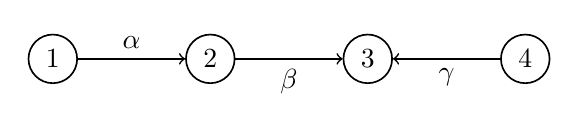
\begin{tikzpicture}[->,-latex, auto, every path/.style={->, semithick}, main node/.style={draw, circle}]
\node	[main node]		(1) at (0,0)		{1};
\node	[main node]		(2) at (2,0)		{2};
\node	[main node]		(3) at (4,0)		{3};
\node [main node]		(4) at (6,0)		{4};

\draw (1) edge node [auto] {$\alpha$} (2);
\draw (2) edge node [auto, swap] {$\beta$} (3);
\draw (4) edge node [auto] {$\gamma$} (3);
\end{tikzpicture}
\eequ
\end{eg}

\begin{mydef}
A \emph{non-trivial path}, $p$, in a quiver is a sequence of arrows $\rho_1, \dots, \rho_n$ which satisfies $t(\rho_{i+1})=s(\rho_i)$ for all $1\leq i <n$, i.e. the start of an arrow is where the previous arrow terminated. The starting and terminatinating vertex of a path $p$ are denoted $s(p)$ and $t(p)$, respectively.
\end{mydef}

\begin{note}
In this report the arrows in a path will be ordered the same way as the composition of functions, as in \cite{CB2}, however, be aware that other publications may order the arrows the opposite way.
\end{note}

\begin{mydef}
The \emph{trivial path} is the path which contains no arrows, i.e. it is a single vertex, and is denoted $e_i$ where the vertex is $i$.
\end{mydef}

\begin{mydef}
The paths of the quiver in Example \ref{ininquivereg} are:
\equ
p_1=e_1, \quad p_2=e_2, \quad p_3=e_3, \quad p_4=e_4, \quad p_5=\alpha, \quad p_6=\beta, \quad p_7=\gamma, \quad p_8=\beta\alpha.
\eequ
However, $\gamma\beta\alpha$ is not a path because $t(\gamma)=3\neq s(\beta)=2$.
\end{mydef}

For the following results we set $A=kQ$ and the $e_i$ are the trivial paths of $Q$.

\begin{lem} 
The $e_i$ are orthogonal, idempotents in $A$, i.e. $e_ie_i=e_i$ and $e_ie_j=0$ where $i\neq j$. Thus $\sum_{i=1}^{n}{e_i}=1_{A}$.
\end{lem}
\begin{proof}
Well, obviously, $e_ie_j=0$ when$i\neq j$ because $t(e_j)\neq s(e_i)$ because they are the trivial paths at different vertices, $i$ and $j$. Similarly, if we have the product $e_ie_i$ then the composition makes sense here because $t(e_i)=s(e_i)$, but the composition is just $e_i$ becuase if we travel along the trivial path $e_i$ twice, then this is just the same as travelling the trivial path 
\end{proof}



\begin{thebibliography}{99}

\bibitem{CB1}
Crawley-Boevey, W.
\emph{Cohomology and Central Simple Algebras}. [Online-PDF file]. [Accessed October 2014].
Available from: http://www1.maths.leeds.ac.uk/~pmtwc/cohom.pdf

\bibitem{CB2}
Crawley-Boevey, W.
\emph{Representation of Quivers}. [Online-PDF file]. [Accessed October 2014].
Available from: http://www1.maths.leeds.ac.uk/~pmtwc/quivlecs.pdf

\bibitem{Rotman}
Rotman, J. J.
2009.
\emph{An Introduction to Homological Algebra}
2nd ed.
New York: Springer Science+Business Media.



\end{thebibliography}


\end{document}
